\documentclass[12pt,letterpaper,noanswers]{exam}
\usepackage[usenames,dvipsnames,svgnames,table]{xcolor}
\usepackage[margin=0.9in]{geometry}
\renewcommand{\familydefault}{\sfdefault}
\usepackage{multicol}
\usepackage{wrapfig}
\pagestyle{head}
\definecolor{c03}{HTML}{FFDDDD}
\header{AM 22b Class 05}{}{Feb 03: vector products}
\runningheadrule
\headrule
\usepackage{graphicx} % more modern
\usepackage{amsmath} 
\usepackage{amssymb} 
\usepackage{hyperref}
\usepackage{tcolorbox}

\usepackage[numbered,autolinebreaks,useliterate]{mcode}

\newcommand{\mb}[1]{\underline{#1}}

\begin{document}
 \pdfpageheight 11in 
  \pdfpagewidth 8.5in


% I need to review the torus trajectories...

\begin{itemize}
% \item There is a pre-class assignment (20 minutes of videos + a few WeBWorK exercises) due at 10am this Monday.  It is available on Canvas.
\itemsep0em
    \item There is a skill check in class on Monday for skill C04 and C05.  The C05 sample problem is at the end of this handout.  Skill checks (and retakes) are done from memory without any aids (notes, calculators, etc).
    \item The C02 / C03 retake will be available on Monday.  It is optional and should be completed for any skill that was not satisfied on the original skill check.
    \item There will be a pre-class assignment due on Monday.
    \item PSet 01 is due on Thursday Feb 4th at 6pm.
    \item PSet 02 will be due on Thursday Feb 11th at 6pm.
\end{itemize}

\hrule
\vspace{0.2cm}



\noindent\textbf{Big picture}

This week we are working with vectors and vector products, with a focus on moving between the algebraic and geometric definitions of the dot product and the cross product.  These vector products will become very important in March: we'll be using them often once we start working with functions that have vectors for their output.
\vspace{0.2cm}
\hrule
\vspace{0.2cm}


\noindent\textbf{Skill Check Practice}

\begin{questions}
\item Let $\mb{u}$ be the vector 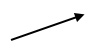
\includegraphics[scale=0.5]{img/C06p1a.png} and $\mb{v}$ be the vector 
\includegraphics[scale=0.5]{img/C06p1b.png}.

Is $\mb{u}\times\mb{v}$ into the page/screen (away from you) or out of the page/screen (towards you)?

\begin{oneparcheckboxes}
\choice into the page
\choice out of the page
\end{oneparcheckboxes}

\item Compute $(2\mb{i}+\mb{j})\times(2\mb{j})$ \textbf{using distributive and scalar multiplication properties} of the cross product along with the cross product relationships between $\mb{i},\mb{j},\mb{k}$.

\framebox(250,30){ cross product:\hfill }
\end{questions}

\vspace{0.2cm}

\hrule
\vspace{0.2cm}

\noindent\textbf{Skill check solution}
\begin{questions}
\item Two options for finding the direction using the right hand rule: 
\begin{itemize}
    \item Draw 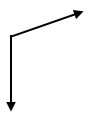
\includegraphics[scale=0.5]{img/C06p1c.png}.  Make a flat hand.  Leave your thumb and index (pointer) finger in place.  Bend your other three fingers towards your palm.  Rotate your hand to align the index finger with the first vector ($\mb{u}$) in such a position that you can also align the other fingers with ($\mb{v})$.  Which way is your thumb pointing?
    \item Draw 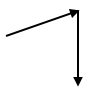
\includegraphics[scale=0.5]{img/C06p1d.png}, with $\mb{u}$ first and $\mb{v}$ drawn from its tip.  Place your palm along $\mb{u}$ oriented so that you can bend your fingers to align with $\mb{v}$.  Which way is your thumb pointing?
\end{itemize}
Your thumb should be into the page/screen in both cases.


    \item Distribute: \begin{align*}
    (2\mb{i}+\mb{j})\times(2\mb{j}) &= (2\mb{i})\times(2\mb{j})+ (\mb{j})\times(2\mb{j}) \\
    &= 4(\mb{i}\times \mb{j})+ 2(\mb{j}\times \mb{j}) \\
    &= 4(\mb{i}\times \mb{j}) \\
    &= 4\mb{k}.
    \end{align*}
%     \item Use determinant notation: \begin{align*}\left\vert\begin{array}{c c c} \mb{i} & \mb{j} & \mb{k} \\ 2 & 2 & 0 \\ 0 & 2 & 0
%     \end{array}\right\vert &= \mb{i}\left\vert\begin{array}{c c}2 & 0 \\ 2 & 0
%     \end{array}\right\vert - \mb{j}\left\vert\begin{array}{c c}2 & 0 \\ 0 & 0
%     \end{array}\right\vert + \mb{k}\left\vert\begin{array}{c c}2 & 2 \\ 0 & 2
%     \end{array}\right\vert \\
%     &= \mb{i}\left(2(0)-0(2)\right)-\mb{j}\left(2(0)-0(0)\right)+\mb{k}\left(2(2)-2(0)\right) \\
%     &= 4\mb{k}
%     \end{align*}
% \end{itemize}
\end{questions}

\vspace{0.2cm}

\hrule
\vspace{0.2cm}


\noindent\textbf{Teams}


New teams today; introduce yourself to your group.

\begin{multicols}{2}

1.  student names

\end{multicols}


\vspace{0.2cm}
\hrule
\vspace{0.2cm}

\noindent\textbf{From C04 Handout:}
\begin{tcolorbox}
The \textbf{dot product} between two vectors of the same size, $\underline{u}$ and $\underline{v}$, is given by $\underline{u}\cdot\underline{v} = u_1v_1+u_2v_2+...+u_nv_n$ where $\underline{u} = (u_1, u_2,...,u_n)^T$ and $\underline{v} = (v_1, v_2, ..., v_n)^T$.  This is the \textbf{algebraic definition} of the dot product.

The \textbf{angle} between the vectors $\underline{u}$ and $\underline{v}$ can be found using the relationship 
$\underline{u}\cdot\underline{v} = \Vert \underline{u}\Vert\Vert\underline{v}\Vert\cos\theta$.  This is the \textbf{geometric definition} of the dot product.
\end{tcolorbox}

\noindent\textbf{Dot product example.}
 Find $\mb{u}\cdot\mb{v}$ where $\mb{u} = 3\mb{i} + \mb{j}-\mb{k}$ and $\mb{v}$ is a vector of length $2$ oriented at an angle of $\pi/4$ away from the direction of $\mb{u}$.
 
 \vspace{1in}

% \vspace{0.2cm}
% \hrule
% \vspace{0.2cm}
% \noindent\textbf{Projected length}
% \begin{tcolorbox}
% Taking a dot product of a vector, $\mb{v}$, with a unit vector, $\hat{\mb{u}}$, gives the \textbf{oriented, projected length} of $\mb{v}$ along the ``\mb{u}-axis''.  \url{https://www.youtube.com/watch?v=LxSMhIUaIc4}
% \end{tcolorbox}

% \noindent\textbf{Example.}
% \begin{itemize}
% \item Let $\mb{v} = 3\mb{i} + 4\mb{j}$ and $\mb{F} = 4\mb{i} + \mb{j}.$  Find the oriented, projected length, of $\mb{F}$ along the direction of $\mb{v}$.
% \vspace{3cm}

% \item Construct a vector $\mb{F}_{\text{parallel}}$ that is parallel to $\mb{v}$, and has its length given by the oriented, projected length, of $\mb{F}$ along the direction of $\mb{v}$.
% \vspace{2cm}
% \end{itemize}




\vspace{0.2cm}
\hrule
\vspace{0.2cm}

\noindent\textbf{Computing the cross product} \S 13.4
\begin{tcolorbox}
The \textbf{cross product} of vectors $\mb{u} = \left(\begin{array}{c} u_1 \\ u_2 \\ u_3 \end{array}\right)$ and $\mb{v} = \left(\begin{array}{c} v_1 \\ v_2 \\ v_3 \end{array}\right)$, denoted $\mb{u}\times\mb{v}$, is \[\mb{u}\times\mb{v} = \left(\begin{array}{c} u_2v_3-u_3v_2 \\ u_3v_1-u_1v_3 \\ u_1v_2 - u_2v_1 \end{array}\right).\]

The cross product is \textbf{anti-commutative}: $\mb{u}\times\mb{v} = -\mb{v}\times\mb{u}$.
\end{tcolorbox}

\noindent\textbf{Example}.
Using the definition above, what is $\vec{i}\times\vec{j}$? What is $\vec{j}\times\vec{i}$?

\vspace{1in}



One way people sometimes remember these relationships is with the following diagram:

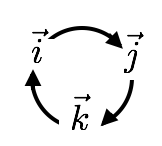
\includegraphics[width=1in]{img/C09ijk.png}

\noindent\textbf{Example}.
Find $\mb{v} \times \mb{v}$.
\vspace{1.2in}

\begin{tcolorbox}
The cross product \textbf{distributes} over addition so $(\mb{u}+\mb{v})\times \mb{w} = \mb{u}\times\mb{w}+\mb{v}\times\mb{w}$.

\textbf{Scalar multiplication} has the following property: $(c\mb{u})\times\mb{v} = \mb{u}\times(c\mb{v}) = c(\mb{u}\times\mb{v})$.
\end{tcolorbox}

\noindent\textbf{Example}.
Find $\mb{v} \times \mb{w}$ with $\mb{v} = 3\mb{i} - 2\mb{j} + 4\mb{k}$ and $\mb{w} = \mb{i} + 2\mb{j} - \mb{k}$ by using the distributive and scalar multiplication properties above, along with the diagram giving the cross product relationships between $\mb{i},\mb{j},\mb{k}$.
\vspace{2in}



\vspace{0.2cm}
\hrule
\vspace{0.2cm}

\noindent\textbf{Cross product geometry} \S 13.4
\begin{tcolorbox}
The cross product $\mb{u}\times\mb{v}$ is \textbf{orthogonal} to $\mb{u}$ and to $\mb{v}$.  \emph{Compute $\mb{u}\cdot(\mb{u}\times\mb{v})$ to convince yourself of this.}

The vector $\mb{u}\times\mb{v}$ points in the direction given by the \textbf{right hand rule} (with $\mb{u}$ playing the role of $x$ and $\mb{v}$ playing the role of $y$ in the $xyz$ coordinate system).

Given three points in a plane that are not co-linear, you can construct two vectors in the plane.  Using the cross product to find a normal vector, you can then construct an equation for the plane.
\end{tcolorbox}

\begin{tcolorbox}
The \textbf{magnitude of the cross product}, $\Vert \mb{u}\times\mb{v}\Vert$ is the area of the parallelogram with edges $\mb{u}$ and $\mb{v}$.

The \textbf{area of the parallelogram} is also given by $\Vert \mb{u}\Vert\Vert\mb{v}\Vert\sin\theta$, where $\theta$ is the angle between the vectors $(0\leq \theta \leq \pi),$ so $\Vert \mb{u}\times \mb{v}\Vert = \Vert\mb{u}\Vert\Vert \mb{v} \Vert \sin \theta$.

The \textbf{area of a triangle} with sides $\mb{u}, \mb{v}, \mb{u}-\mb{v}$ is given by $\frac{1}{2}\Vert\mb{u}\times\mb{v}\Vert.$




\end{tcolorbox}

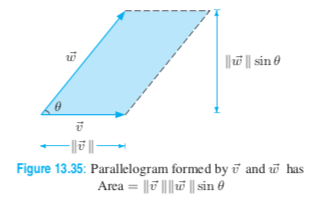
\includegraphics[scale=0.7]{img/C05parallelogram.png}

\noindent\textbf{Example.} Let points $(0,1,2)$, $(2,-1,3)$ and $(0,0,1)$ form a triangle that lies in a plane.
\begin{itemize}
    \item Find a normal vector to the plane, and construct an equation for the plane
    \vspace{1.5in}
    
   % \item Construct an equation for the plane.
    \item Find the area of the triangle. 
    \vspace{0.5in}
    % and construct an area vector for it.
   % \item Construct an area vector for the triangle.
\end{itemize}





\vspace{0.2cm}
\hrule
\vspace{0.2cm}


%{\sc Add a wireframe flat surface approximation thing where you've used the cross product to find area vectors for all of the parallelograms...  And pick a hard cross product Q from the text so that we can practice starting hard problems.}

\noindent\textbf{Question}.

Figure 13.44 shows the tetrahedron determined by three vectors $\mb{a}, \mb{b}, \mb{c}$.

\begin{tcolorbox}
The \textbf{area vector} of a face is a vector perpendicular to the face, pointing outward, whose magnitude is the area of the face. 
\end{tcolorbox}

We want to show that the sum of the four outward pointing area vectors of the faces equals the zero vector.  

\noindent Discuss how to approach this problem.

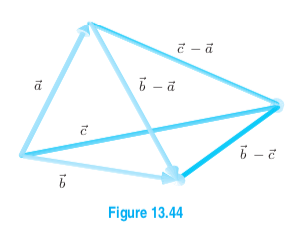
\includegraphics[scale=0.4]{img/C05tetrahedron.png}

\vspace{0.2cm}
\hrule
\vspace{0.2cm}


\noindent\textbf{Review questions}

\begin{questions}
\item True or False (discuss): There is only one point in the $yz$-plane that is distance $5$ from the point $(3,0,0)$.
\item Explain what is wrong with the statement: A contour diagram for $z = f(x,y)$ is a surface in $xyz$-space.
\item Explain what is wrong with the statement: The functions $f(x,y) = \sqrt{x^2+y^2}$ and $g(x,y) = x^2+y^2$ have the same contour diagram.
\end{questions}

\end{document}